\documentclass[11pt,a4paper]{jsarticle}
%

\usepackage{amsmath,amssymb}
\usepackage{bm}
\usepackage[dvipdfmx]{color}
\usepackage[dvipdfmx]{graphicx}
\usepackage{ascmac}
\usepackage{listings, jlisting}
\lstset{%
  basicstyle={\small},%
  identifierstyle={\small},%
  commentstyle={\small\itshape},%
  keywordstyle={\small\bfseries},%
  ndkeywordstyle={\small},%
  stringstyle={\small\ttfamily},
  frame={tb},
  breaklines=true,
  columns=[l]{fullflexible},%
  numbers=none,%
  xrightmargin=0zw,%
  xleftmargin=3zw,%
  numberstyle={\scriptsize},%
  stepnumber=1,
  numbersep=1zw,%
  lineskip=-0.5ex%
}


%
\setlength{\textwidth}{\fullwidth}
\setlength{\textheight}{40\baselineskip}
\addtolength{\textheight}{\topskip}
\setlength{\voffset}{-0.2in}
\setlength{\topmargin}{0pt}
\setlength{\headheight}{0pt}
\setlength{\headsep}{0pt}

%
\newcommand{\divergence}{\mathrm{div}\,}  %ダイバージェンス
\newcommand{\grad}{\mathrm{grad}\,}  %グラディエント
\newcommand{\rot}{\mathrm{rot}\,}  %ローテーション
%
\title{チャレンジサイト・メカニックカモノハシ2019\\マイクロマウスシミュレータExercise}
\author{ER17045 立道壱太郎}
\date{\today}
\begin{document}
\maketitle
%
%
\section{この資料について}
メカニックカモノハシではマイクロマウス大会に参加することでメンバーの技術向上を図ります。


\section{マイクロマウスパッケージの導入}

\subsection{workspaceの作成}
メカニックカモノハシ用のworkspaceを新たに作りましょう。

\begin{lstlisting}[frame=single, caption=workspaceの作成, label=create_workspace]
$ mkdir -p ~/mp_ws/src
$ cd ~/mp_ws/src/
$ catkin_init_workspace
$ echo "source ~/mp_ws/devel/setup.bash" >> ~/.bashrc
\end{lstlisting}


\subsection{マイクロマウスパッケージの導入}
githubから、パッケージをcloneしてcatkin\_makeします。
\begin{lstlisting}[frame=single, caption=catkin\_make, label=catkin_make]
$ cd ~/mp_ws/src
$ git clone https://github.com/platypus5384/micro_mouse.git
$ cd ~/mp_ws
$ catkin_ws
$ source ~/.bashrc
\end{lstlisting}

以下のコマンドを入力し、ディレクトリを移動できれば成功です。
\begin{lstlisting}[frame=single, caption=roscd, label=roscd]
$ roscd micro_mouse
\end{lstlisting}


\newpage

\section{関連パッケージの導入}
マイクロマウスパッケージの動作に必要な関連パッケージを導入します。
以下のコマンドを実行してください。(全部で一行)
\begin{lstlisting}[frame=single, caption=roscd, label=roscd]
sudo apt install ros-kinetic-turtlebot ros-kinetic-turtlebot-msgs ros-kinetic-turtlebot-teleop 
\end{lstlisting}

\section{micro\_mouse動作テスト}
付いていると思いますが、一応、ファイルに権限を付けます。以下を実行してください。
\begin{lstlisting}[frame=single, caption=roscd, label=roscd]
$ roscd micro_mouse/script
$ sudo chmod -R a+x *
\end{lstlisting}

シミュレータを起動します。以下のコマンドをそれぞれ別端末で実行してください。
\begin{lstlisting}[frame=single, caption=roscd, label=roscd]
$ roslaunch micro_mouse startup.launch
別の端末を開き、
$ rosrun micro_mouse left_hund_ex.py
\end{lstlisting}


マウスが動き出し、マッピングが始まれば成功です。
しばらく待つと、以下のようになります。
\begin{figure}[h]
  \begin{center}
    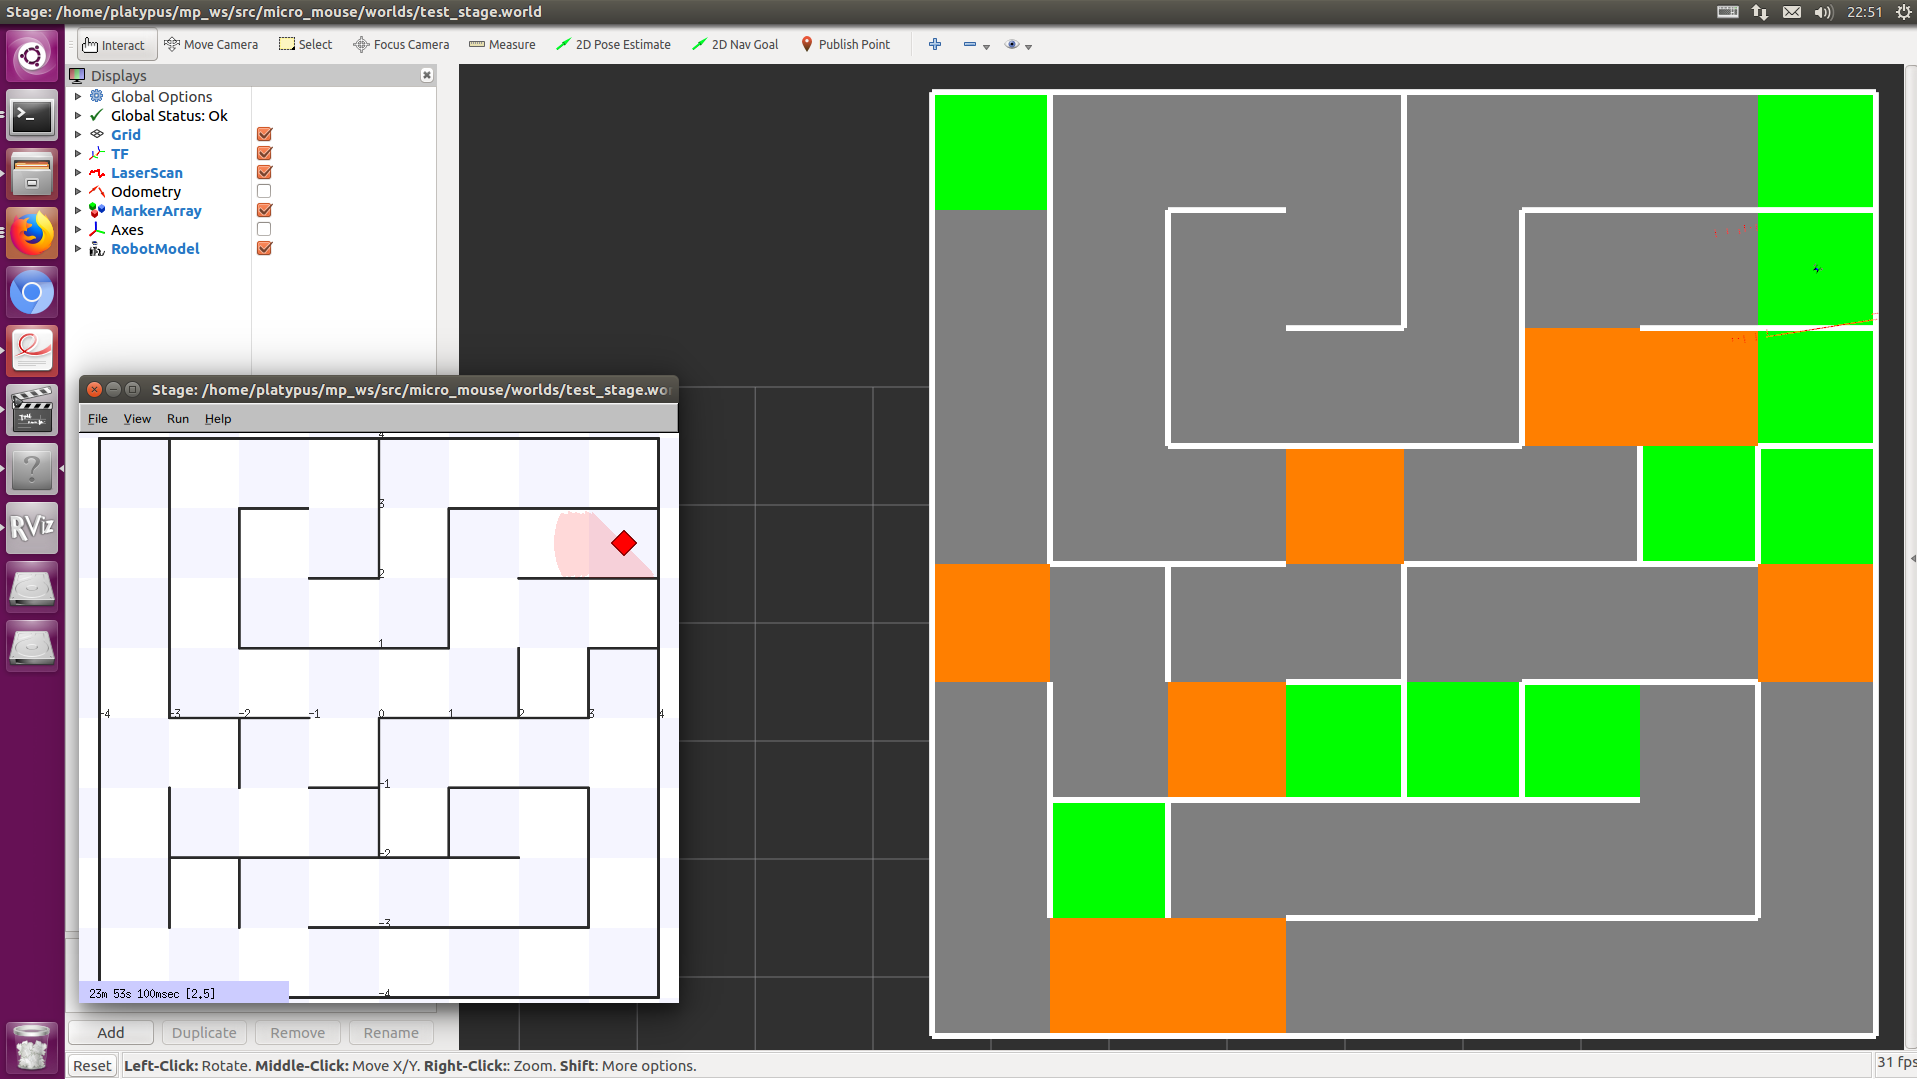
\includegraphics[width=128mm]{./mms_test.png}
  \end{center}
  \caption{}
  \label{graph3}
\end{figure}




\section{Exercise}
\subsection{Python簡易入門}
簡易的にPython入門しよう。

\newpage
\subsection{マウスを動かそう}

\lstinputlisting[caption=micro\_mouse/script/chapter/1/moving\_mouse.py,label=moveing_mouse,numbers=left]{./../../script/chapters/1/moving_mouse.py}


\newpage
\lstinputlisting[caption=micro\_mouse/script/chapter/1/going\_mouse.py,label=going_mouse,numbers=left]{./../../script/chapters/1/going_mouse.py}


\newpage
\lstinputlisting[caption=micro\_mouse/script/chapter/1/sensing\_mouse.py,label=sensing_mouse,numbers=left]{./../../script/chapters/1/sensing_mouse.py}




\newpage
\subsection{wallPublisherを使いこなそう}




\newpage
\subsection{pathPublisherを使いこなそう}




\newpage
\subsection{左手法・拡張左手法・足立法を理解しよう}
\subsubsection{左手法}
\lstinputlisting[caption=micro\_mouse/script/chapter/3/left\_hund.py,label=left_hund,numbers=left]{./../../script/chapters/3/left_hund.py}


\newpage
\subsubsection{拡張左手法}
\lstinputlisting[caption=micro\_mouse/script/chapter/3/left\_hund\_ex.py,label=left_hund_ex,numbers=left]{./../../script/chapters/3/left_hund_ex.py}


\subsubsection{足立法}





\newpage
\subsection{経路計画を理解しよう}



%\lstinputlisting[caption=moving\_mouse.py,label=moveing_mouse,numbers=left]{./../script/chapters/1/moving_mouse.py}


\begin{thebibliography}{99}
\bibitem{install_ubuntu16} Windows10とUbuntu16.04のデュアルブート環境構築\\https://qiita.com/medalotte/items/4bb5cfa709e93d044f1c
\bibitem{install_ubuntu18} Windows10とUbuntu18.04をデュアルブートする.\\https://qiita.com/yo\_kanyukari/items/2a944a300db22482c696
\end{thebibliography}%
%
\end{document}
